\documentclass[border=10pt]{standalone}

\usepackage{tikz}
\usepackage{tikzsymbols}
\usetikzlibrary{calc,patterns,shapes.geometric}

\def\centerarc[#1](#2)(#3:#4:#5){\draw[#1] ($(#2)+({#5*cos(#3)},{#5*sin(#3)})$) arc (#3:#4:#5);}

\begin{document}
	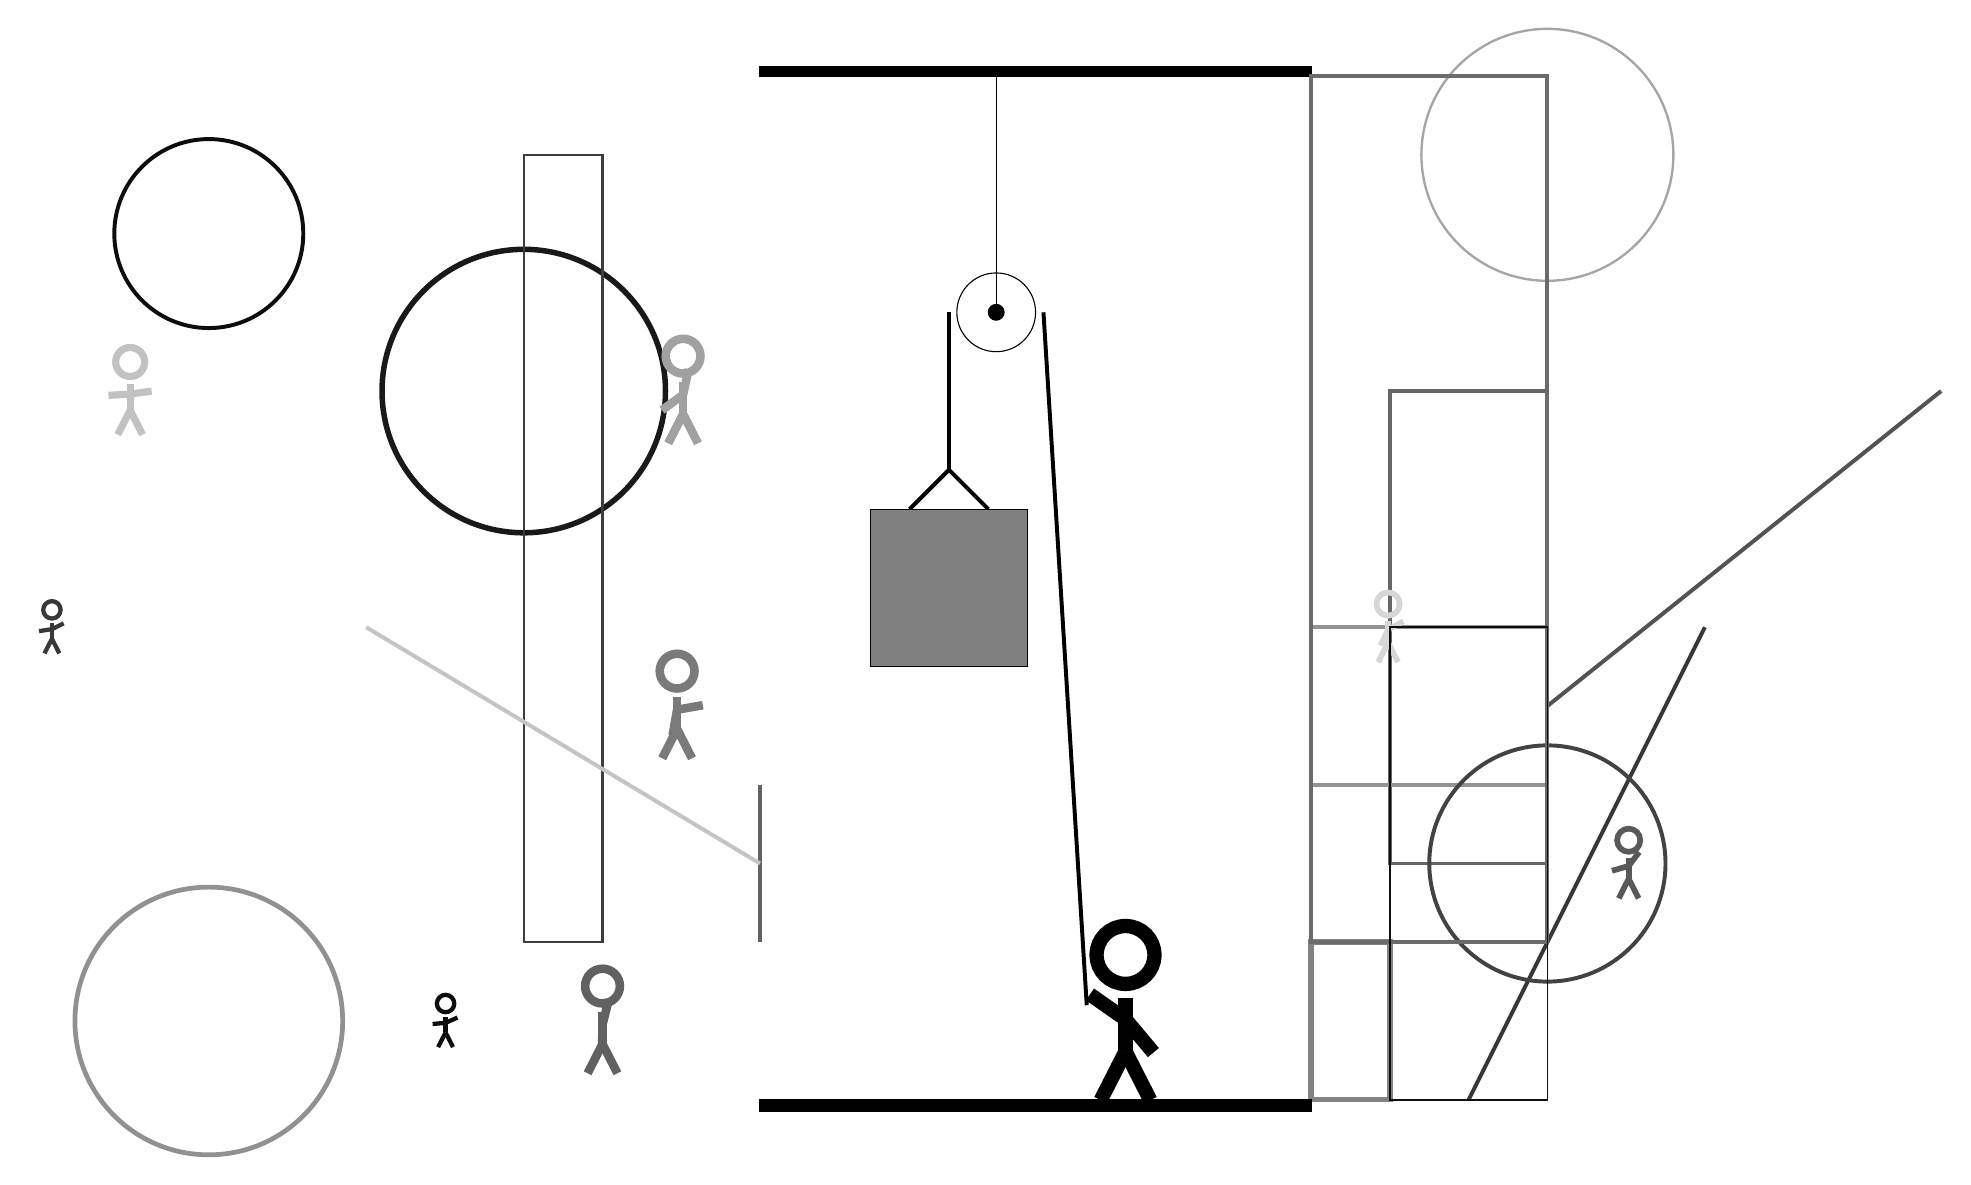
\begin{tikzpicture}
		%%%%% START %%%%%
		
		\draw[fill=black] (-2, 10) rectangle (5, 10.125);
		
		\draw (1, 7) circle (0.5);
		\draw[fill=black] (1, 7) circle (0.1);
		\draw (1, 10) -- (1, 7);
		
		\draw[line width=0.5mm] (-0.1, 4.5) -- (0.4, 5.0) -- (0.9, 4.5);
		\draw[fill=black!50] (-0.6, 4.5) rectangle (1.4, 2.5);
		
		\node[line width=0.4mm, color=black!52] at (-3, 2) {\Strichmaxerl[6][80][10]};
		
		\draw[line width=0.7mm, color=black!49] (5, -3) rectangle (6, -1);
		\draw[line width=0.5mm, color=black!60] (6, 6) rectangle (8, 0);
		\draw[line width=0.5mm, color=black!61](-2, 1) -- (-2, -1);
		\node[line width=0.5mm, color=black!95] at (-6, -2) {\Strichmaxerl[3][5][24]};
		\draw [line width=0.5mm, color=black!61](-11, 6) circle (0.0);
		\draw [line width=0.7mm, color=black!90](-5, 6) circle (1.8);
		\draw[line width=0.3mm, color=black!76] (-4, 9) rectangle (-5, -1);
		\node[line width=0.6mm, color=black!78] at (-11, 3) {\Strichmaxerl[3][9][26]};
		
		\node[line width=0.5mm, color=black!62] at (-4, -2) {\Strichmaxerl[6][89][76]};
		\draw[line width=0.5mm, color=black!42] (5, 3) rectangle (8, 1);
		\draw[line width=0.5mm, color=black!78](7, -3) -- (10, 3);
		\node[line width=0.2mm, color=black!37] at (-3, 6) {\Strichmaxerl[6][36][78]};
		\draw [line width=0.3mm, color=black!35](8, 9) circle (1.6);
		\node[line width=0.6mm, color=black!16] at (6, 3) {\Strichmaxerl[4][64][29]};
		\draw[line width=0.5mm, color=black!68](8, 2) -- (13, 6);
		\draw [line width=0.5mm, color=black!74](8, 0) circle (1.5);
		\draw[line width=0.5mm, color=black!23](-7, 3) -- (-2, 0);
		\draw [line width=0.5mm, color=black!95](-9, 8) circle (1.2);
		\node[line width=0.4mm, color=black!65] at (9, 0) {\Strichmaxerl[4][16][53]};
		\draw[line width=0.5mm, color=black!58] (5, -1) rectangle (8, 10);
		
		\draw[line width=0.2mm, color=black!94] (6, -3) rectangle (8, 3);
		
		\draw [line width=0.6mm, color=black!43](-9, -2) circle (1.7);
		\node[line width=0.2mm, color=black!24] at (-10, 6) {\Strichmaxerl[5][3][8]};
		
		\draw[line width=0.5mm] (0.4, 7) -- (0.4, 5.0);
		\centerarc[line width=0.5mm](1, 7)(0:180:0.6);
		\draw[line width=0.5mm](1.6, 7) -- (2.15, -1.8);
		
		\node at (2.6, -1.9) {\Strichmaxerl[10][-35][-50]};
		
		\draw[fill=black] (-2, -3) rectangle (5, -3.15);
		
		%%%%% END %%%%%
	\end{tikzpicture}
\end{document}